\documentclass[a4paper]{article}

%% Language and font encodings
\usepackage[english]{babel}
\usepackage[utf8x]{inputenc}
\usepackage[T1]{fontenc}


%% Sets page size and margins
\usepackage[a4paper,top=3cm,bottom=2cm,left=3cm,right=3cm,marginparwidth=1.75cm]{geometry}

%% Useful packages
\usepackage{amsmath}
\usepackage{graphicx}
\usepackage[colorinlistoftodos]{todonotes}
\usepackage[colorlinks=true, allcolors=blue]{hyperref}

\usepackage{fancyhdr}
\setlength{\headheight}{15.2pt}
\pagestyle{fancy}
\lhead{A Study On Global Warming}
\rhead{J.~Book, E.~Jakobsson, S.~Gabrielli}

\usepackage{float}

\usepackage{epstopdf}

\title{Global Warming Project}
\author{Edvin Jakobsson, Johan Book, Sara Gabrielli}

\begin{document}
\begin{titlepage}
	\begin{flushright}
		2017-11-09\\
	\end{flushright}
	\vfill
	\begin{center}
		{\huge\bf An Emphasis on Global Warming 
		\\[3mm] 
		\large Using Geographical Weather Data
		}
		\\[3cm]
		{Edvin Jakobsson, Johan Book, Sara Gabrielli}
		\\[5mm]
		{Department of Astronomy and Theoretical Physics, Lund University}
		\\[2cm]
		{MNXB01}

		\vfill
		
\includegraphics[height=6cm]{logo_no_text.png}
	\end{center}
\end{titlepage}

\tableofcontents

\newpage
\section{Introduction}

A hot topic today is that of man-made global warming, and it is sometimes described as one of the greatest threats that mankind has ever faced. Our collective impact on our planet has grown immensely over the last century, and the effects are starting to show all over the world. However, the changes seems rather humble still, and our complacency constrains us from acting appropriately. At first glance it may seem like we have far more pressing issues, but in the end it could very well be our inability to care for our planet that determines our extinction.

\medskip
\medskip
The long-term effects on the surface-temperature of the Earth is not detectable from day to day, but studying data covering decades one could clearly witness a systematic increase in temperature. The Swedish Meteorological and Hydrological Institute (SMHI) recently published records of daily temperature measurements in the Swedish city of Uppsala dating all the way back to the year 1722. By analyzing this data it is possible to detect increases in the average temperature over centuries, as well as many other interesting phenomena.

\medskip
\medskip
This project focuses on studying three related topics, the behavior of temperature averages in different areas in Sweden, the distribution of the hottest and coldest day of the year over time, and the increase of the average temperature in Uppsala over the last couple of centuries.

\section{Method}\label{sec:Methods}

\subsection{Data and \texttt{ROOT} version used}
The project relies on data files from SMHI and H.~Bergström and A.~Moberg \cite{Uppsala}. Boras, Falsterbo, Falun, Karlstad, Luleå, Lund, Söderarm, Umeå and Uppsala. All data files, except for Uppsala, features data from the latest century. However, the data from Uppsala ranges back to 1722.
\linebreak
The \texttt{ROOT} version 5.34/30 was used to analyze data.

% Johan Book
\subsection{Yearly Average Temperature Over Different Places}

The code reads all data files from SMHI and for each file it creates, using C++ in ROOT, an average for each year (including calculation of standard deviation). Each file was plotted separately using continuous error-bars. By creating a semi-transparent overlay\footnote{This was done in Inkscape due to an incompatibility between OpenGL and ROOT.} a single graph, vaguely describing the general properties of the system could be constructed.

\medskip
\medskip
The code utilized a class \texttt{treader} which parses a data file into a set of instances of \texttt{tpoint}, each containing an entry consisting of date and temperature.


\subsection{Hottest and Coldest days and overall trend of the temperatures}\label{sec:Saras method}

In order to create histograms, showing when the warmest and coldest days typically occurred from $1722$ up to $2013$ in Uppsala, two
arrays respectively storing the hottest and coldest day for each year are needed. The code \texttt{Sara{\_}Producefiles.cpp} was written in order to read the data of
the SMHI recorded from Uppsala and then produce two output files:
\begin{itemize}
\item one file called \texttt{year\_hotday\_coldday.dat}, containing a list of the years with the corresponding hottest and coldest days; 
\item a second file called \texttt{years\_days\_temps.dat}, containing most of the recorded temperatures (the criterion for the exclusion of some temperatures is explained below) with the corresponding day 
(from 1 to 366) and year.
\end{itemize}
\medskip
Since not all the data contained in the file from the SMHI were  recorded from the same place, all the readings from a region other
than Uppsala should be ignored. In the first output file the code returns $0$  for the years in which no temperature was measured in Uppsala (and also for the corresponding hottest and coldest days). In the second output file a line of "$0$" is present for each temperature not recorded in the region of interest.

\medskip
\medskip
The data from the Uppsala.dat file are read into a two-dimensional array. The functions \texttt{Function{\_}max} and \texttt{Function{\_}min} are used inside a loop over the first column of the array (containing all the years associated to the temperatures recorded in the 
SMHI file) in order to find the hottest temperature and the coldest temperature of each year with the associated days. The maximization
and minimization are achieved by comparing each temperature with the one stored in the following line, so that the higher/lower temperature between the two is written over the one previously stored in the variable \texttt{Tmax\_temporary} or \texttt{Tmin\_temporary}. The two functions store temperature and day in an array and return the pointer to the array. The function \texttt{NumberoutofDate}
is used in the two functions mentioned above and, if the two-dimensional array and the line of the hottest/coldest temperature
are passed, it returns a number between 1 and 366 corresponding to the day in which that specific temperature has been recorded. 

\medskip

The loop cycle in which the functions mentioned above are called produces an array containing a list of the years, and two arrays containing the hottest and coldest days respectively. These three arrays are printed in the first output file of the code.
The arrays needed to produce the second output file are generated in the second loop of the code.

\medskip
\medskip

A ROOT macro \texttt{Sara{\_}Analyze.C}  was then written in order to read the files produced by the first code and store the data of each column in a different array, but excluding the lines containing $0$ in the first column. An array is produced by the macro for each column of the two files and the so obtained arrays are exploited for producing graphs and histograms.

\medskip
\medskip
Two overlaying histograms are produced by calling the class \texttt{TH1} : one for the distribution of the hottest days and one showing the distribution of the coldest days. The histogram for the hottest days is fitted with a Gaussian function and the mean of the distribution is returned with its uncertainty in order to predict when the hottest day is more likely to occur. The second histogram is fitted with two Gaussian functions since the coldest days mainly occur both at the end of the year and at the beginning. The hottest and coldest days are
plotted either against the years in which thy occur in two separate graphs, by calling the class \texttt{TGraph}.

\medskip
\medskip

The \texttt{2DGraph} class in ROOT is used to obtain two different views of the three-dimensional graph showing how the temperatures in Uppsala changed over the days of the years from 1722 to 2013.The option \texttt{Draw("surf1")} is used to obtain a graph as the one showed in fig.\ref{fig:3D}. The option \texttt{Draw("colz")} is used to obtain a view from the top of the graph.

\subsection{Global Warming}

A script called \texttt{global\_warming.C} was written C++, and was later executed in ROOT. The function \texttt{global\_warming()} included the classes \texttt{treader} and \texttt{tpoint} which were used to read the data provided. Three arguments were required, a path to the data file, a starting year and an end year for the analyzation. The function then read through the data and calculated an average temperature for each year. A total average for all the used data was also calculated. Two histograms were then created, one colored red which contained all years above the total average and one colored blue which contained all years below the total average. Two moving averages were also calculated with a step length of 5 and 10 years, using the average of the years in a vicinity of 5 or 10 years respectively. The function then created a picture containing both histograms and graphs of moving averages, and saved it on the computer.


\section{Results}\label{sec:Results}

% Johan Book
\subsection{Average Yearly Temperature Over Distinct Places}

The produced figure (see figure \ref{fig:johan}) represents the distributions of average temperature for different years (y-axis) and different places (distinct colors). The darker areas correspond to regions shared by several places. Cities included in the figure are; Boras, Falsterbo, Falun, Karlstad, Luleå, Lund, Söderarm and Umeå.

\begin{figure}[H]
\begin{center}
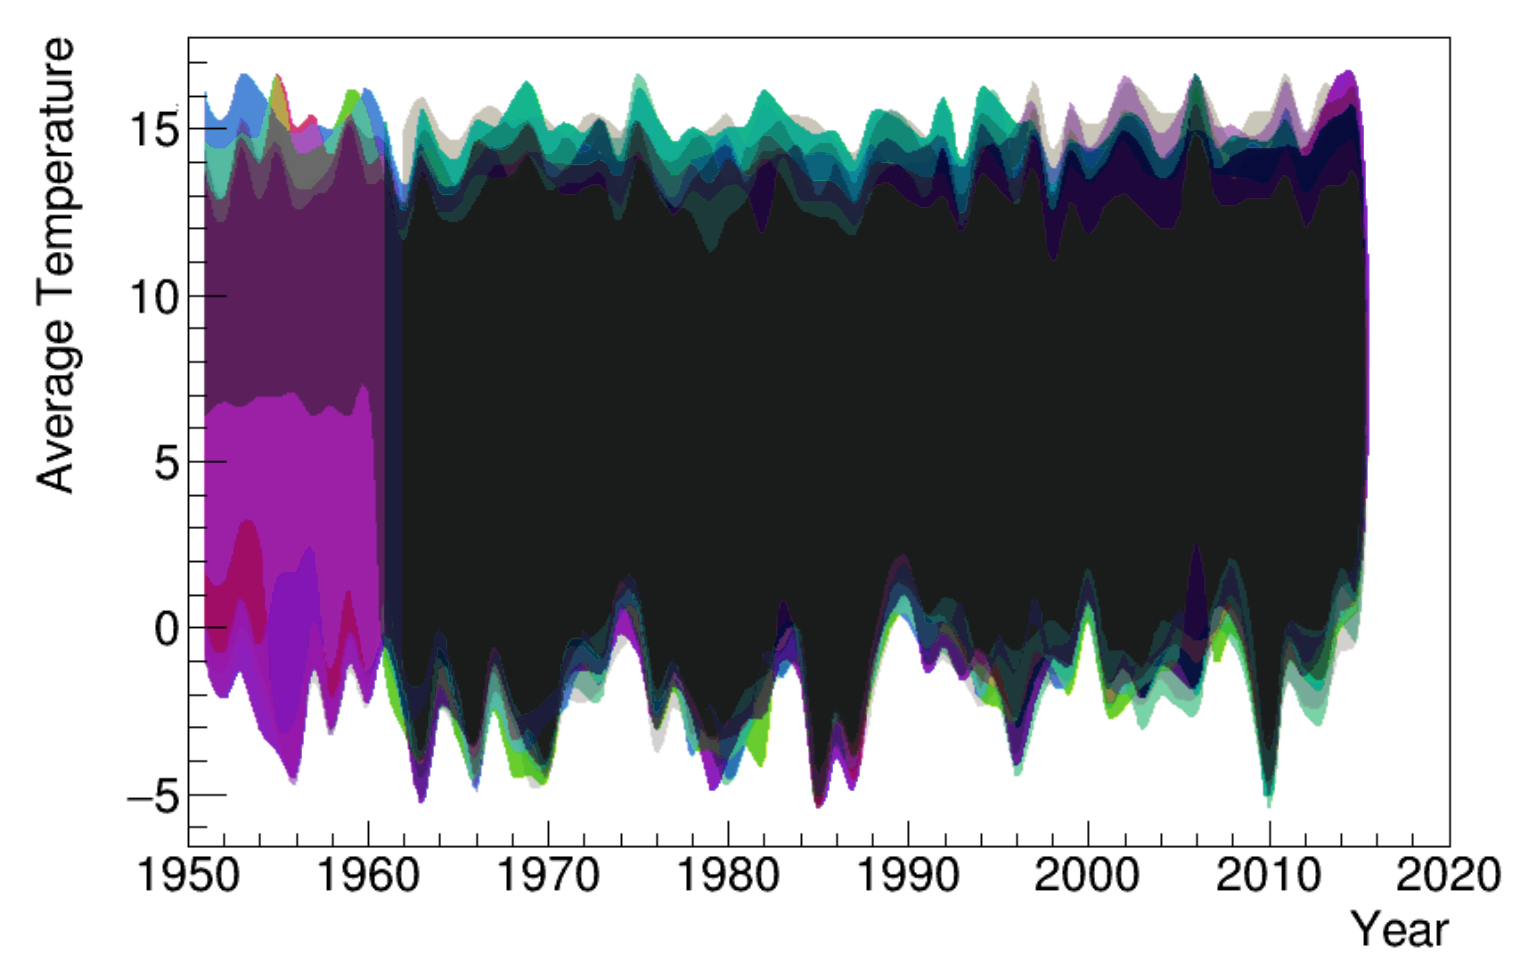
\includegraphics[scale=.3]{2.png}
\caption{The yearly average temperature including error. Different cities uses distinct color. Darker areas correspond the regions shared among several places. Note the cyclic tendency of the lower boundary.}
\label{fig:johan}
\end{center}
\end{figure}


\subsection{Hottest and Coldest days and overall trend of the temperatures}

The overlaying histograms showing the distribution of the hottest and the coldest days are shown in figure \ref{fig:HotColdHist}.
The mean obtained for the distribution of the hottest days is $193 \pm 2$. The graphs showing how the hottest days and coldest days changed over the years are shown in figures  \ref{fig:HotGraph} and \ref{fig:ColdGraph}. 


\begin{figure}[H]
\begin{center}
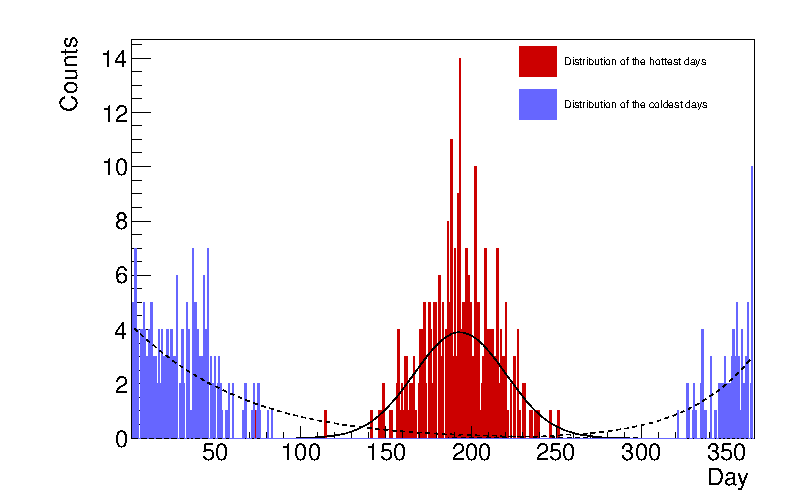
\includegraphics[width=0.9\textwidth]{HottestColdest.png}
\caption{Histogram showing how often each day of the year was the warmest or coldest from 1722 to 2013. Lines show Gaussian fits of the two distributions.}
\label{fig:HotColdHist}
\end{center}
\end{figure}

\begin{figure}[H]
\begin{center}
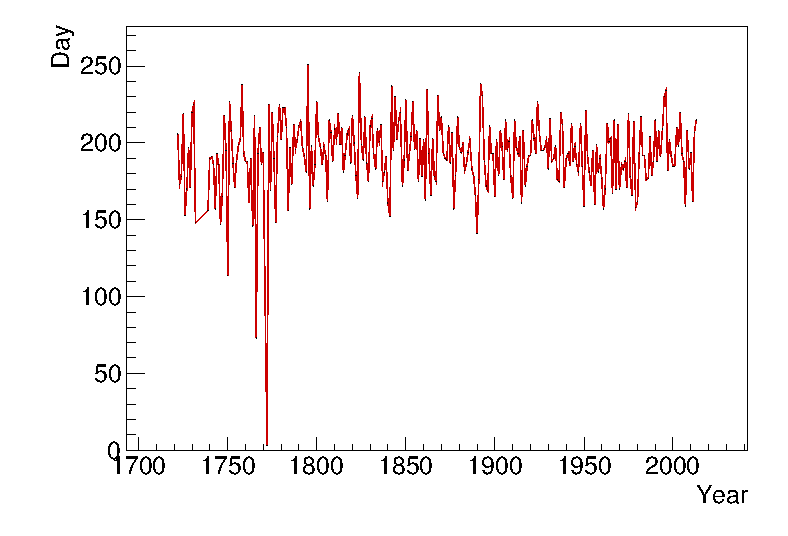
\includegraphics[width=13cm]{graph1DHot.png}
\caption{Graph showing the hottest day for each year from 1722 to 2013.}
\label{fig:HotGraph}
\end{center}
\end{figure}

\begin{figure}[H]
\begin{center}
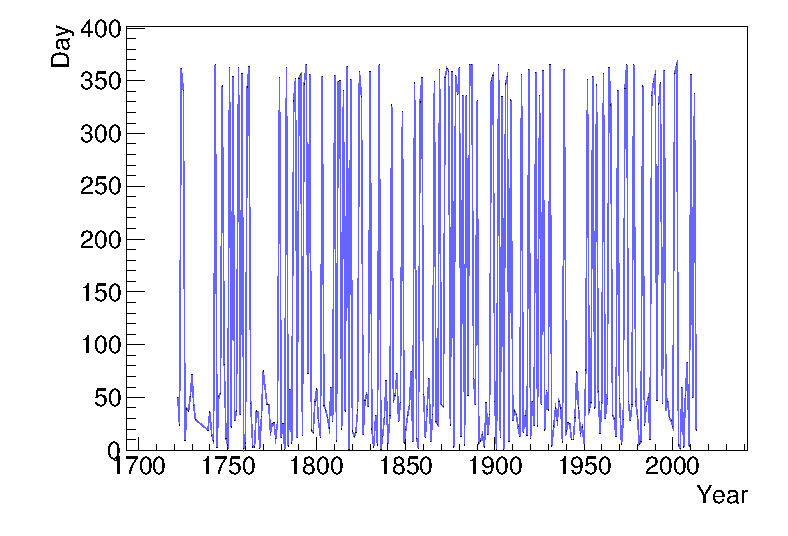
\includegraphics[width=11cm]{graph1D.png}
\caption{Graph showing the coldest day for each year from 1722 to 2013.}
\label{fig:ColdGraph}
\end{center}
\end{figure}

\begin{figure}[H]
\begin{center}
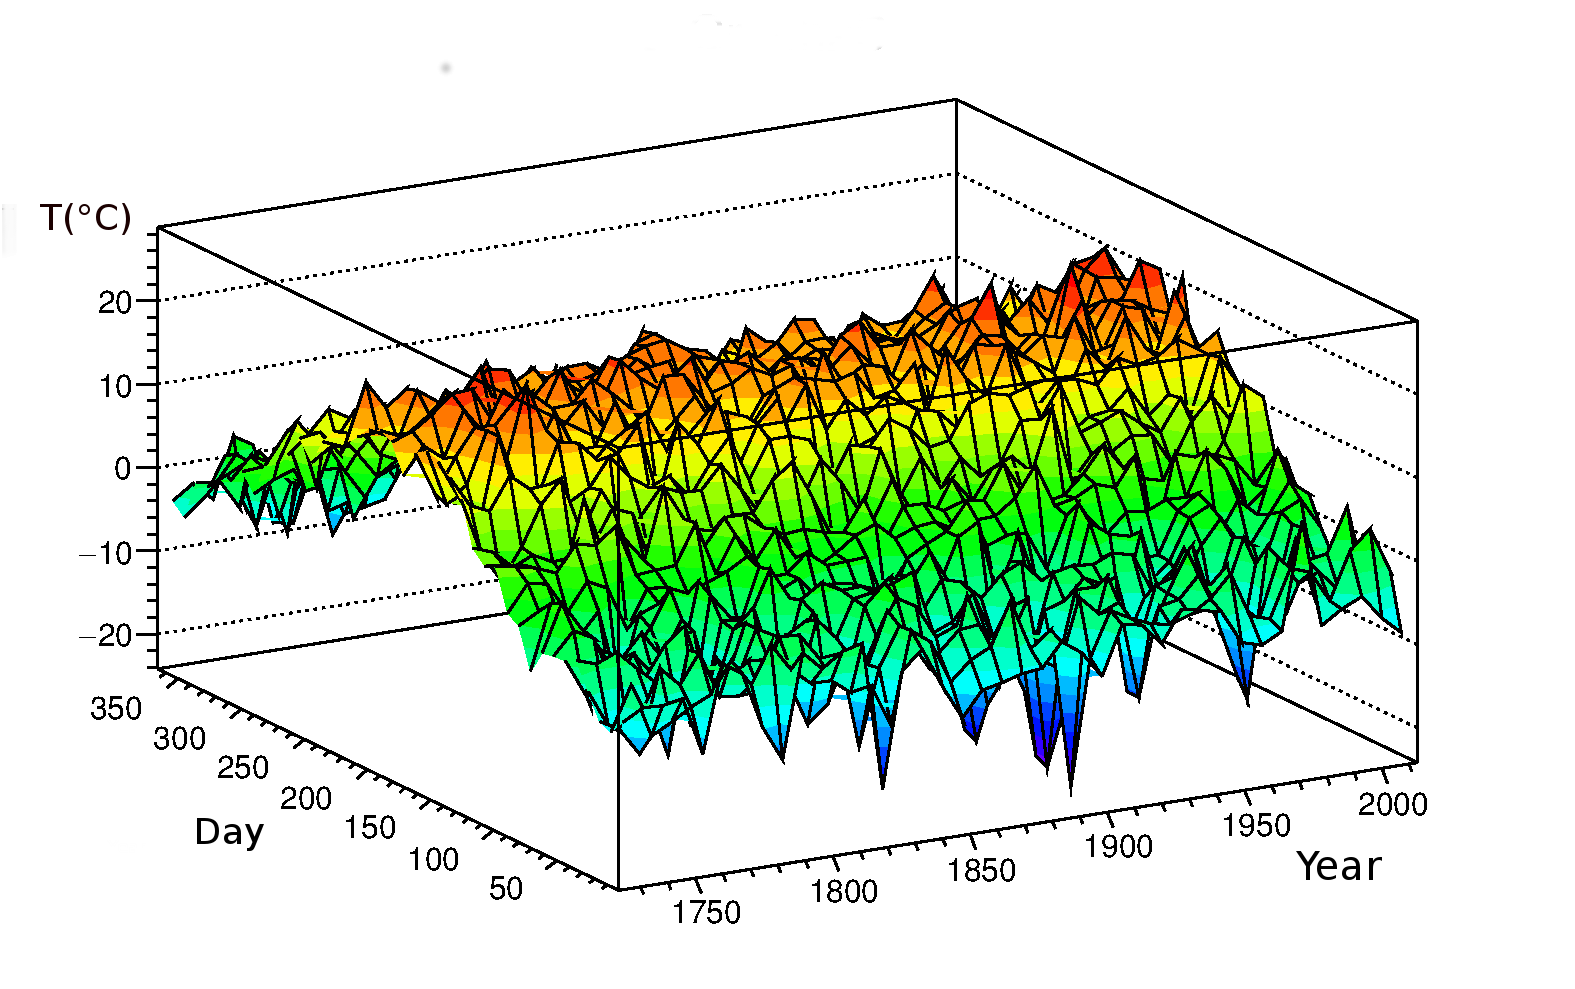
\includegraphics[width=0.9\textwidth]{2Dgraph1.png}
\caption{Graph showing how the temperatures in Uppsala changed over the days of the years from 1722 to 2013.}
\label{fig:3D}
\end{center}
\end{figure}

\begin{figure}[H]
\begin{center}
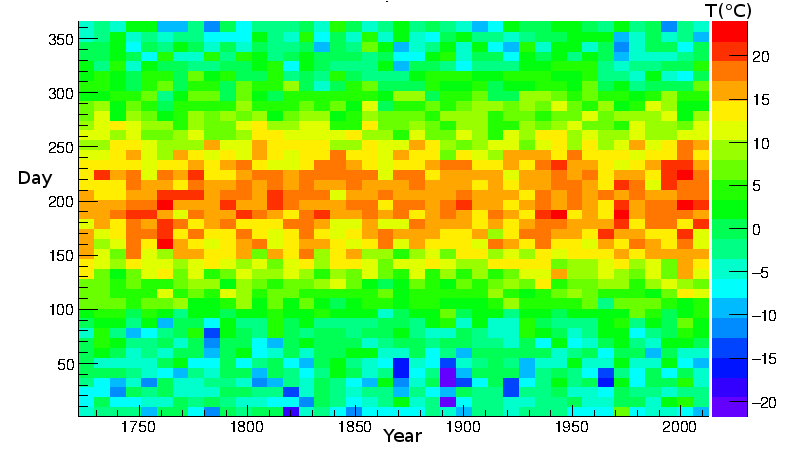
\includegraphics[width=11cm]{2Dgraphint.png}
\caption{View from the top of the Graph in figure \ref{fig:3D}.}
\label{fig:top3D}
\end{center}
\end{figure}


\subsection{Global Warming}

The script \texttt{global\_function.C} was used with all the data contributed from Uppsala, i.e. temperature measurements from 1722 to 2013. A histogram including all the data was then created, see figure \ref{global_warming_figure}. The average temperature of each year was displayed as a bin stretching from the total average of approximately $ 5.5 \hspace{1mm} ^\circ C$. Red bins were used for bins with temperatures above the total average and blue bins were used otherwise. On top of this two graphs were created to show two types of moving averages. The first graph displayed an average calculated every 5 years by including the next and the previous 5 years. The second graph was instead calculated every 10 years and included the next and the previous 10 years. This graph was drawn with a thicker line in order to separate the two.

\begin{figure}[H]
\centering
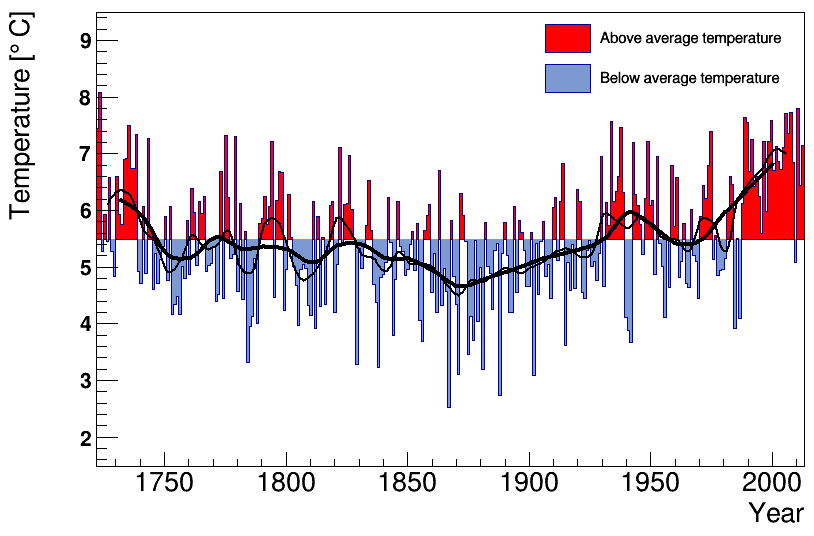
\includegraphics[width=0.8\textwidth]{global_warming.png}
\caption{\label{global_warming_figure} The average temperature of each year in Uppsala. A total average was calculated as approximately $5.5 \hspace{1mm} ^\circ C$ and each average temperature is displayed as either a red bin, if the temperature is above the total average, or a blue bin, if the temperature is below the total average. Two black graphs displays moving averages. The thinner line describes the average in the vicinity of 5 years and the thicker line the vicinity of 20 years. Note that the average temperature of the last 20 years is disturbingly high. }
\end{figure}


\section{Discussion}\label{sec:Discussion}

% Johan Book  #Chicken chicken chicken chicken chicken. Chickens? Chickens! All them chickens!
\subsection{Yearly Average Temperature For Distinct Places}

Figure \ref{fig:johan} shows several interesting phenomena.
The top border does not show any direct patterns, however, the lower border does. Firstly, one can observe some form of cycle where the temperature is temporarily increased during a period roughly every five years. Secondly, one can see a slight hint of an overall temperature increase. However, whether it is a natural occurrence or not cannot be determined from this figure alone.

\subsection{Hottest and Coldest days and overall trend of the temperatures}
Figure \ref{fig:HotColdHist} shows that the hottest temperature in Uppsala is most likely to be registered around the day $193$ (corresponding to July 12 on a regular year). Despite the fitting with Gaussian functions, it is not possible to determine an average of the distribution of the coldest days since it is split into two parts at the beginning and at the end of the year. Consequently another histogram, which is shown in figure \ref{fig:HotColdHist2}, has been obtained where the left part of the histogram (from day 1 to 99) is shifted to the right ( so that the days from 1 to 99 in the first histogram in figure \ref{fig:HotColdHist} correspond to the days from 376 to 465 in figure \ref{fig:HotColdHist2}). In this way we can notice that the mean of the Gaussian function fitting the histogram of the coldest days in figure \ref{fig:HotColdHist2} is 383, and thus the coldest temperature is most likely to be measured in the day number 17 (January 17) with an uncertainty of 3 days.

\begin{figure}[H]
\begin{center}
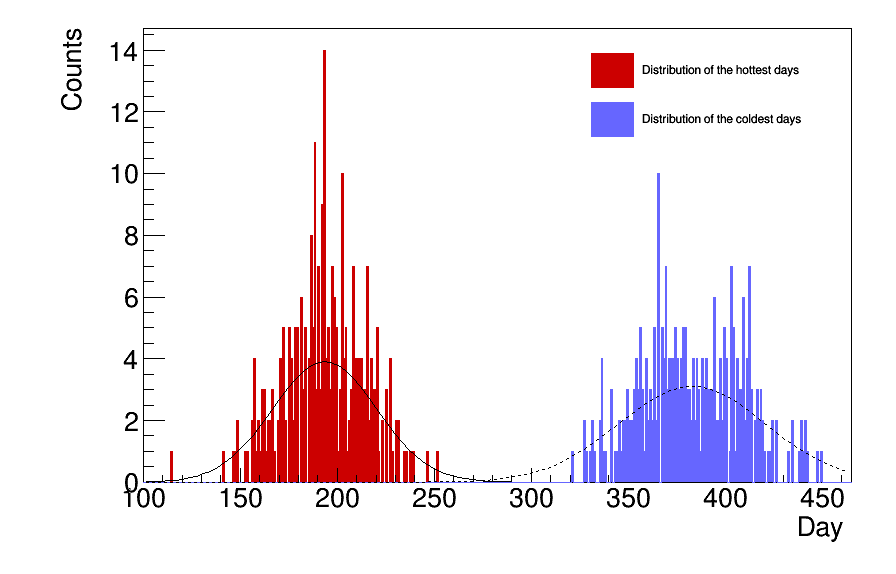
\includegraphics[width=0.7\textwidth]{HotCold_shifted.png}
\caption{"Shifted histogram" obtained by moving the left part of figure \ref{fig:HotColdHist} to the right.}
\label{fig:HotColdHist2}
\end{center}
\end{figure}


Figures \ref{fig:HotColdHist} and \ref{fig:HotGraph} besides show some unexpected values for the hottest days. This is due to the exclusion of some temperatures as described in section
\ref{sec:Saras method}. For some of the years most (and sometimes all) of the temperatures were recorded from regions
different from Uppsala and this implies that for those years less days were candidate for being the hottest or the coldest. 

\medskip
\medskip
The aim of the three-dimensional graph was to point out eventual modifications in the seasonal change, for example a shift in the start of summer. However, none of these changes were observed and apparently the effect of global warming is not evident either. This result might appear contradictory to what we obtained in figure \ref{global_warming_figure}, but this is maybe due to two factors:
\begin{itemize}
\item a change of about $2 \hspace{1mm} ^\circ C$ is not observable in the color coding used for the temperature in figure \ref{fig:top3D};
\item while in figure \ref{global_warming_figure} average temperatures are considered for each year, in the three-dimensional graphs all the daily temperatures are considered.
\end{itemize}


\subsection{Global Warming}

It is quite evident from the histogram (see figure \ref{global_warming_figure}) that the average temperature (at least in Uppsala) can vary a lot from one year to the next. Over decades, however, we can see a shift between warmer and colder periods, and even clearer so if we observe the moving averages. The nineteenth century seem to have been quite a cold period in Sweden, with the average temperature dropping to almost one degree below the total average. The early eighteenth century may seem to indicate a higher average, but this is mostly due to that the years 1722 to 1735 were all quite warm, and the moving average has no data prior to 1722 to use. It is hence unclear whether the average temperature of the eighteenth century was much higher than that of the following century, and the moving averages might be a bit misleading in this regard.

\medskip
\medskip
From the histogram it is more evident that the average temperature since the start of the twentieths century has increased. The average temperature between 1970 and 2010 is more than a degree higher than that of the period between 1870 and 1910. This does not prove any form of man-made global warming, but it is a strong indication that the surface-temperature of the Earth is increasing. There is however other research showing that the human way of life is a big factor in this global warming.

\section{Conclusion}



The results derived in this report are indecisive but hints that global warming could be real. An increase in the average temperature over the last century is clearly visible, however the cause of this increase is not accounted for. No shift in the hottest or coldest day of the year was observable, hinting at that this is not affected by the average temperature.

\medskip
\medskip
However disturbing the fact is that most of the hottest years in several centuries are all found after the year 1990, it is not evident from this research alone that the effect is man-made. Further investigation on this subject is required.

% The Bibliography
\begin{thebibliography}{9}
\bibitem{github}
Book, J., Jakobsson E., Gabrielli S. : 
\textit{The MNXB01 Project} (2017)\\
https://github.com/JohanBook/MNXB01-Project

\bibitem{Uppsala}
Bergström, H., Moberg, A. :
    \textit{Daily air temperature and pressure series for Uppsala} (1722-1998), 
    Climate Change, 53:213-252.

\end{thebibliography}

\end{document}